In diesem Abschnitt werden die Direct Cascade Netzwerke jeweils einmal mit und einmal ohne Transfer Learning evaluiert. Im Vergleich zu den 
bisherigen Experimenten erfolgt das Training mit einer deutlich erhöhten Anzahl an Netzwerkiterationen innerhalb der Kaskade, wobei die Anzahl der 
Epochen pro Einzelnetzwerk konstant bleibt. Für alle Tests wird ausschließlich eine geringe Menge an Target-Daten verwendet.

\begin{figure}[htpb]
    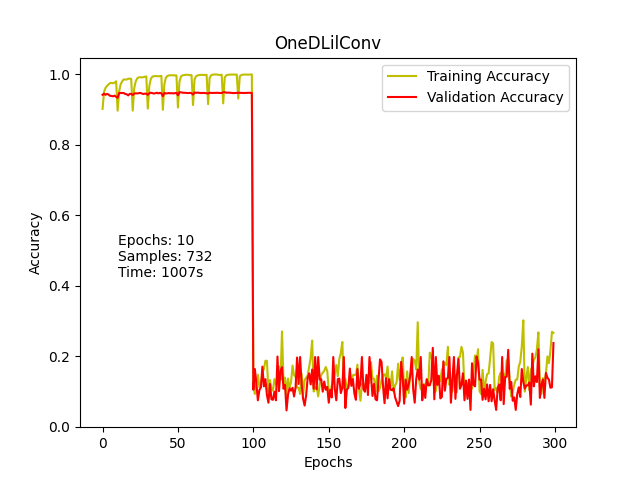
\includegraphics[height=5cm]{../../Plots/ba_plots/classTF/1dc_tr.png}
    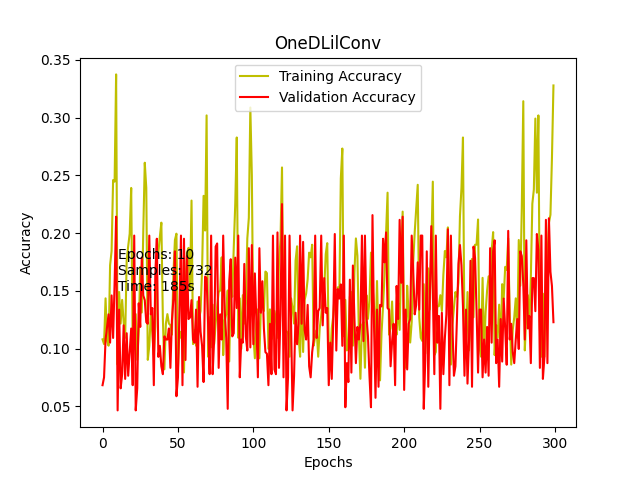
\includegraphics[height=5cm]{../../Plots/ba_plots/classTF/wo1dc_tr.png}
    \caption{\label{fig:1dc_tr} 
    \small{In der Abbildung sind links die Ergebnisse des Tests 1DC:TF10/732/10/30 und rechts jene des Tests 1DC:732/10/30 dargestellt. Die 
    Variante mit TF weist eine deutlich längere Trainingszeit auf, was auf die Größe des verwendeten Sourcedatensatzes zurückzuführen ist. In 
    beiden Fällen zeigt sich jedoch, dass die Netzwerke unabhängig vom Einsatz von TF eine insgesamt geringe Performanz aufweisen.}}
\end{figure}

Wie in Abbildung \ref{fig:1dc_tr} ersichtlich, besteht kein signifikanter Unterschied in der Accuracy zwischen den 
Modellen mit und ohne TF in den Convolutional Layern. In beiden Fällen bleibt die Leistung auf einem sehr niedrigen Niveau, was 
sich ebenfalls in den Testergebnissen widerspiegelt.

\begin{figure}[htpb]
    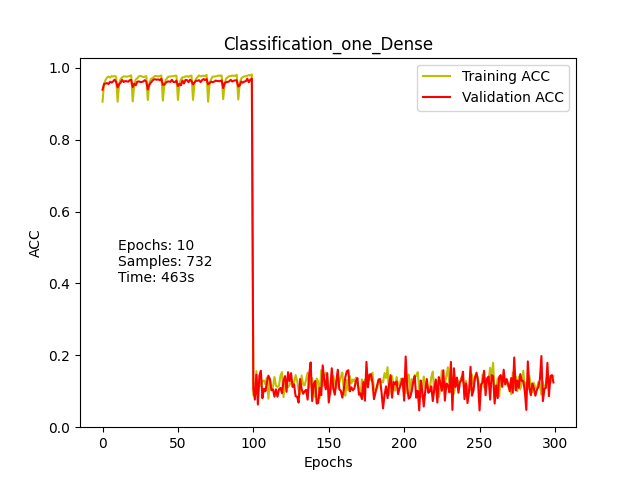
\includegraphics[height=5cm]{../../Plots/ba_plots/classTF/cod_tr.png}
    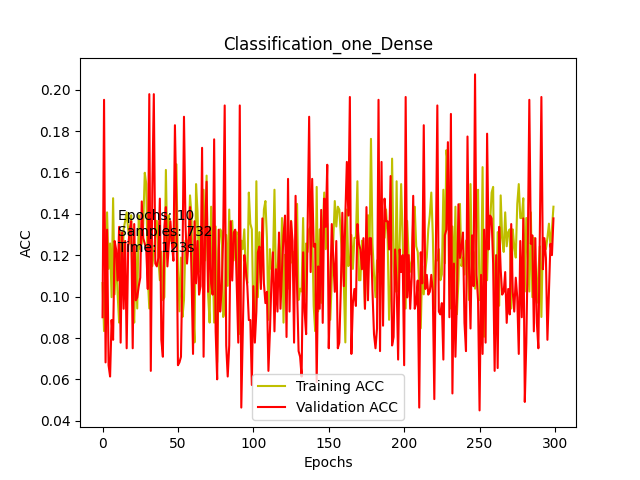
\includegraphics[height=5cm]{../../Plots/ba_plots/classTF/wocod_tr.png}
    \caption{\label{fig:cod_tr} 
    \small{Links ist das Testergebnis des Experiments COD:TF10/732/10/30 dargestellt, bei dem TF eingesetzt wurde, rechts jenes des 
    Experiments COD:732/10/30 ohne TF. Auch in diesem weiteren Fall, bei dem die Architektur mit Linearen Schichten als Hidden Layer verwendet 
    wurde, zeigen sich unabhängig vom Einsatz von TF ebenfalls geringe Leistungswerte.}}
\end{figure}

Das beobachtete Rauschen in den Darstellungen resultiert daraus, dass nach jeweils zehn Epochen ein neues Netzwerk initialisiert und trainiert 
wird. Obwohl das Wissen der zuvor trainierten Netzwerke über die Eingabedaten verfügbar ist, wird dieses nicht unmittelbar durch optimale 
Gewichtungen transferiert.

Abbildung \ref{fig:cod_tr} zeigt ein vergleichbares Ergebnis, basierend auf linearen Schichten. Für dieses Verhalten kommen zwei Ursachen in 
Betracht: Zum einen könnte das Kaskadieren der Netzwerke nicht wie vorgesehen funktionieren, zum anderen könnte eine unzureichende Menge an 
Target-Daten vorliegen. Letzteres wurde bereits in vorangegangenen Untersuchungen überprüft und führte zwar zu einer Verbesserung, jedoch 
bleiben die Resultate weiterhin nur moderat.

Diese Beobachtungen legen nahe, dass insbesondere beim Kaskadieren der Netzwerke Schwierigkeiten bestehen.
